% !TeX program = pdflatex
%==============================================================================
%  Aula 05 --- Árvores de Regressão e Ensembles
%  VERSÃO DO ALUNO: texto para leitura autônoma, fora da sala.
%  (O roteiro de sala é "06 Arvores de Regressao e Ensembles.tex".)
%
%  A figura da partição/árvore usa os cortes de uma árvore REAL de profundidade 2
%  (n=300, dados em [0,10]^2, R^2 = 0,941). Ver o comentário antes dela.
%==============================================================================
\documentclass[11pt,a4paper]{article}
\usepackage[aluno]{../../recursos/latex/estilo-notas}

\title{}
\date{}

\begin{document}
\cabecalhoaula{05}{Árvores de Regressão e \emph{Ensembles}}{AME §4.8--4.10; ISLP cap.~8}

%==============================================================================
\section*{O que você vai aprender}
%==============================================================================
Ao final desta aula você deve ser capaz de:
\begin{itemize}[leftmargin=1.4cm]
  \item descrever como uma \textbf{árvore de regressão} particiona o espaço de
        covariáveis e prediz por médias locais;
  \item explicar a construção em duas etapas: \emph{crescimento} por divisões
        binárias recursivas e \emph{poda} por custo--complexidade;
  \item justificar, via redução de variância, por que \textbf{agregar} estimadores
        ajuda;
  \item descrever \textbf{bagging}, a estimativa \emph{out-of-bag} e a medida de
        importância de variáveis;
  \item explicar como as \textbf{florestas aleatórias} \emph{descorrelacionam} as
        árvores e o papel de $m$;
  \item descrever \textbf{boosting} como ajuste incremental dos resíduos e o papel
        de $\lambda$, $B$ e da profundidade.
\end{itemize}

\noindent
Árvores são o método mais \emph{interpretável} que veremos --- e, sozinhas, das
piores em predição. A história desta aula é como transformá-las, por agregação, em
alguns dos métodos \emph{mais poderosos} que existem para dados tabulares
(florestas, XGBoost). A pergunta que organiza tudo:

\begin{center}\itshape
  como combinar muitos modelos ruins para obter um ótimo?
\end{center}

\noindent
A resposta tem nome e sobrenome --- Proposição~\ref{prop:media} --- e duas condições.
Cada método desta aula é uma tentativa de satisfazer melhor a segunda delas.

%==============================================================================
\section{Árvores de regressão}
%==============================================================================
Uma árvore parte o espaço de covariáveis em regiões disjuntas $R_1,\dots,R_J$ por
\emph{particionamento recursivo} e prediz, em cada região, a média das respostas de
treino ali contidas:
\begin{equation}\label{eq:arvore}
  g(\x) = \frac{1}{\abs{\{i:\X_i\in R_k\}}}\sum_{i:\X_i\in R_k} Y_i,
  \qquad \text{para } \x\in R_k .
\end{equation}
Para prever, percorre-se a árvore do topo às folhas seguindo as condições
(``$x_j<t$?'') em cada nó.

% ---------------------------------------------------------------------------
% Cortes reais: DecisionTreeRegressor(max_depth=2) sobre n=300 pontos uniformes
% em [0,10]^2, com y = 4,5 / 3,0 / 2,5 / 0,5 conforme a região + ruído N(0;0,35^2).
% Árvore obtida:  x1 <= 3,99 ? -> (x2 <= 6,09 ? 2,97 : 4,49) : (x2 <= 2,96 ? 2,50 : 0,52)
% R^2 no treino = 0,941.
% ---------------------------------------------------------------------------
\begin{figure}[htbp]
  \centering
  \begin{tikzpicture}[font=\small]
    % ---------- painel esquerdo: a partição do plano ----------
    \begin{scope}[x=0.50cm, y=0.50cm]
      \fill[azulufrj!16] (0,0) rectangle (3.99,6.09);
      \fill[vinho!22]    (0,6.09) rectangle (3.99,10);
      \fill[verdeesc!18] (3.99,0) rectangle (10,2.96);
      \fill[cinzaclaro]  (3.99,2.96) rectangle (10,10);
      \draw[very thick]  (3.99,0) -- (3.99,10);
      \draw[thick]       (0,6.09) -- (3.99,6.09);
      \draw[thick]       (3.99,2.96) -- (10,2.96);
      \draw (0,0) rectangle (10,10);
      \node at (2.0,3.0)  {$R_1$};   \node[font=\scriptsize] at (2.0,2.1) {$2{,}97$};
      \node at (2.0,8.0)  {$R_2$};   \node[font=\scriptsize] at (2.0,7.1) {$4{,}49$};
      \node at (7.0,1.5)  {$R_3$};   \node[font=\scriptsize] at (7.0,0.7) {$2{,}50$};
      \node at (7.0,6.5)  {$R_4$};   \node[font=\scriptsize] at (7.0,5.6) {$0{,}52$};
      \node[below] at (5,-1.35) {$x_1$};
      \node[rotate=90] at (-1.7,5) {$x_2$};
      \node[font=\scriptsize,below] at (3.99,-0.1) {$3{,}99$};
      \node[font=\scriptsize,left]  at (-0.15,6.09) {$6{,}09$};
      \node[font=\scriptsize,right] at (10.1,2.96) {$2{,}96$};
    \end{scope}

    % ---------- painel direito: a árvore ----------
    \begin{scope}[xshift=9.6cm, yshift=4.1cm,
                  no/.style={draw,azulufrj,rounded corners=2pt,inner sep=2.5pt,
                             font=\footnotesize,fill=white},
                  folha/.style={draw,inner sep=2.5pt,font=\footnotesize},
                  aresta/.style={-,gray!70}]
      \node[no] (raiz) at (0,0) {$x_1 \le 3{,}99$};
      \node[no] (e)  at (-1.9,-1.3) {$x_2 \le 6{,}09$};
      \node[no] (d)  at ( 1.9,-1.3) {$x_2 \le 2{,}96$};
      \node[folha,fill=azulufrj!16] (f1) at (-2.9,-2.7) {$2{,}97$};
      \node[folha,fill=vinho!22]    (f2) at (-1.0,-2.7) {$4{,}49$};
      \node[folha,fill=verdeesc!18] (f3) at ( 1.0,-2.7) {$2{,}50$};
      \node[folha,fill=cinzaclaro]  (f4) at ( 2.9,-2.7) {$0{,}52$};
      \draw[aresta] (raiz) -- node[above left,font=\tiny] {sim} (e);
      \draw[aresta] (raiz) -- node[above right,font=\tiny] {não} (d);
      \draw[aresta] (e) -- node[left,font=\tiny] {sim} (f1);
      \draw[aresta] (e) -- node[right,font=\tiny] {não} (f2);
      \draw[aresta] (d) -- node[left,font=\tiny] {sim} (f3);
      \draw[aresta] (d) -- node[right,font=\tiny] {não} (f4);
      \foreach \px/\rot in {-2.9/1, -1.0/2, 1.0/3, 2.9/4}
        \node[font=\scriptsize,gray] at (\px,-3.4) {$R_\rot$};
    \end{scope}
  \end{tikzpicture}
  \caption{Os dois lados da mesma coisa. À esquerda, a partição de $[0,10]^2$ em
  quatro retângulos; à direita, a árvore que a produz. Cada nó interno é um corte
  perpendicular a um eixo, cada folha é uma região, e o número na folha é a média
  \eqref{eq:arvore} das respostas de treino ali. Os valores são de um ajuste real
  ($n=300$, profundidade~2, $R^2=0{,}941$ no treino). Repare que o corte de
  $x_2$ é \emph{diferente} nos dois ramos ($6{,}09$ à esquerda, $2{,}96$ à direita):
  é assim que a árvore captura uma interação sem que ninguém a tenha especificado.}
  \label{fig:particao}
\end{figure}

\begin{ideia}
Vantagens estruturais das árvores: (i) altamente \textbf{interpretáveis};
(ii) lidam \emph{nativamente} com covariáveis discretas (cortes do tipo
$x_j\in\{\text{verde},\text{vermelho}\}$ --- sem precisar criar \emph{dummies});
(iii) fazem \textbf{seleção de variáveis} automática; (iv) capturam
\textbf{interações} sem que precisemos especificá-las.
\end{ideia}

\begin{atencao}[e a desvantagem estrutural]
Os cortes são sempre \emph{perpendiculares aos eixos}. Uma fronteira diagonal
simples, como $x_1+x_2 > 10$, obriga a árvore a aproximá-la por uma escadinha de
muitos cortes --- e cada degrau custa dados. Se você suspeita de relações lineares
nas covariáveis, um modelo linear (Aula~02) faz melhor com muito menos.
\end{atencao}

\subsection{Etapa 1 --- crescimento (divisões binárias recursivas)}
Idealmente escolheríamos a partição que minimiza o EQM
$P(T)=\sum_R\sum_{i:\X_i\in R}(Y_i-\widehat y_R)^2/n$. Mas buscar a árvore ótima é
computacionalmente inviável (NP-difícil). Usa-se então uma heurística
\emph{gananciosa}: a cada passo, escolhe-se a covariável $x_j$ e o corte $t$ que
mais reduzem a soma de quadrados ao dividir uma região em
$R_1=\{x_j<t\}$ e $R_2=\{x_j\ge t\}$:
\begin{equation}\label{eq:split}
  \min_{j,\,t}\ \sum_{i:\X_i\in R_1}(Y_i-\widehat y_{R_1})^2
            + \sum_{i:\X_i\in R_2}(Y_i-\widehat y_{R_2})^2 .
\end{equation}
Repete-se recursivamente em cada região-filha, até um critério de parada (ex.: menos
de 5 observações por folha). Isso gera uma árvore grande $T_0$, que ajusta bem o
treino mas tende a \textbf{superajustar}.

\begin{observacao}
``Ganancioso'' quer dizer que a escolha de \eqref{eq:split} olha \emph{um passo}
à frente e nunca volta atrás: o primeiro corte é o que mais reduz o RSS agora, ainda
que outro corte pior agora permitisse cortes muito melhores depois. Não é um defeito
de implementação --- é o preço de fugir de um problema NP-difícil. Guarde isso: parte
do ganho dos \emph{ensembles} vem justamente de compensar essa miopia.
\end{observacao}

\begin{observacao}[o tamanho da miopia, medido]\label{obs:miopia}
Vale saber quanto isso custa, porque é mais do que parece. Tome
$y=\operatorname{sinal}(x_1x_2x_3)$ em $[-1,1]^3$: oito regiões resolvem o problema
\emph{exatamente}, e caberiam numa árvore de profundidade~3. A §3 da \texttt{Aula
prática 06} mede o que a árvore gananciosa faz com ele:

\begin{itemize}[leftmargin=1.2cm,nosep]
  \item o primeiro corte reduz $0{,}194\%$ do RSS, e o segundo, $0{,}350\%$ --- a
        cegueira \textbf{não} é só do primeiro passo, porque os oito octantes
        continuam se cancelando dois a dois depois de qualquer corte;
  \item o $R^2$ de teste é \textbf{negativo} até a profundidade~5, isto é, pior que
        chutar a média; encosta em $0{,}17$ na~6 e só chega a $0{,}87$ com a árvore
        cheia, de 59 folhas.
\end{itemize}

Ela precisa gastar cinco níveis de cortes inúteis antes de as regiões ficarem
pequenas o bastante para o sinal aparecer. A mesma seção do notebook mede o caso de
duas dimensões, $y=\operatorname{sinal}(x_1x_2)$, em que basta \emph{um} corte às
cegas: cada dimensão a mais custa um nível inteiro de cegueira.

E há um corolário prático que vale mais que o exemplo. Se você tentar economizar
cortes com um critério de parada precoce --- \texttt{min\_impurity\_decrease=0,005},
digamos --- a árvore fica com \textbf{uma folha}: o critério nunca vê meio por cento
de redução em lugar nenhum, e desiste antes de começar. É por isso que se cresce a
árvore inteira e \emph{depois} se poda, que é o assunto da próxima subseção.
\end{observacao}

\subsection{Etapa 2 --- poda por custo--complexidade}
Para reduzir a variância, \emph{podamos} $T_0$. A poda por custo--complexidade
introduz um parâmetro $\alpha\ge 0$ e busca a subárvore $T\subseteq T_0$ que
minimiza
\begin{equation}\label{eq:poda}
  \sum_{k=1}^{\abs{T}}\sum_{i:\X_i\in R_k}(Y_i-\widehat y_{R_k})^2
   + \alpha\,\abs{T},
\end{equation}
onde $\abs{T}$ é o número de folhas. O termo $\alpha\abs{T}$ penaliza árvores
grandes --- é exatamente a mesma estrutura da regularização da Aula~02, com
$\abs{T}$ no papel de $\norm{\bbeta}_1$: ajuste $+$ $\lambda\times$ complexidade.
$\alpha$ é o \textbf{tuning parameter}, escolhido por \textbf{validação cruzada}
(Aula~03): $\alpha=0$ devolve $T_0$; $\alpha\to\infty$ colapsa para a raiz
(média global).

\begin{atencao}
Crescer e podar usam objetivos diferentes \emph{de propósito}: cresce-se de forma
gananciosa (olhando só um passo à frente) e corrige-se globalmente na poda. Não
confunda profundidade máxima (parâmetro de crescimento) com $\alpha$ (parâmetro de
poda) --- ambos controlam complexidade, mas em etapas distintas.
\end{atencao}

%==============================================================================
\section{Por que agregar? Redução de variância}
%==============================================================================
Árvores isoladas têm \emph{alta variância}: pequenas mudanças nos dados mudam
bastante a árvore --- basta que o corte da raiz mude um pouco para que toda a
estrutura abaixo dele seja outra. A ideia dos \emph{ensembles} é \textbf{combinar}
muitas funções para reduzir essa variância.

\begin{proposicao}[Média de preditores reduz o risco]\label{prop:media}
Sejam $g_1,\dots,g_B$ estimadores \emph{não-viesados}
($\E[g_b(\x)]=r(\x)$), de mesma variância $v(\x)=\Var(g_b(\x))$ e
\emph{não-correlacionados}. Então a média $\bar g=\frac1B\sum_b g_b$ tem risco
\[
  \E[(Y-\bar g(\x))^2\mid\x] = \Var(Y\mid\x) + \frac{v(\x)}{B}
  \;\le\; \E[(Y-g_b(\x))^2\mid\x].
\]
\end{proposicao}
\begin{proof}
Pela decomposição viés--variância (Aula~01), o risco de qualquer preditor $g$ é
$\Var(Y\mid\x)+\mathrm{viés}^2+\Var(g(\x))$. Como cada $g_b$ é não-viesado, $\bar
g$ também é (viés $=0$). Para a variância, sendo os $g_b$ não-correlacionados e de
variância $v(\x)$,
$\Var(\bar g(\x))=\frac1{B^2}\sum_b \Var(g_b(\x))=v(\x)/B$. Substituindo obtém-se a
igualdade; como $v(\x)/B\le v(\x)$, o risco não aumenta.
\end{proof}

\begin{ideia}
Duas exigências da Prop.~\ref{prop:media} guiam tudo o que segue: precisamos de
preditores (i) \textbf{não-viesados} --- por isso usamos árvores \emph{não podadas}
(profundas, baixo viés) --- e (ii) \textbf{pouco correlacionados} --- o ponto fraco,
que as florestas aleatórias atacam diretamente.
\end{ideia}

\begin{observacao}[o que acontece quando a hipótese falha]
A hipótese de não-correlação é forte demais para ser verdade, e vale saber o preço.
Se as $g_b$ têm correlação $\rho$ duas a duas, a conta vira
\[
  \Var(\bar g(\x)) = \rho\, v(\x) + \frac{1-\rho}{B}\,v(\x)
  \ \xrightarrow[B\to\infty]{}\ \rho\,v(\x).
\]
Ou seja: por mais árvores que você acrescente, a variância \textbf{não desce abaixo
de $\rho\,v(\x)$}. O termo que $B$ mata é só o segundo. É por isso que reduzir
$\rho$ vale mais do que aumentar $B$ --- e é literalmente essa a ideia das florestas
aleatórias.
\end{observacao}

%==============================================================================
\section{Bagging}
%==============================================================================
\emph{Bagging} (\emph{bootstrap aggregating}) gera diversidade reamostrando os
dados. Para $b=1,\dots,B$: sorteie uma amostra \textbf{bootstrap} (com reposição,
tamanho $n$) e ajuste nela uma árvore \emph{profunda} (não podada) $g_b$. A predição
é a média:
\begin{equation}\label{eq:bagging}
  g(\x) = \frac1B\sum_{b=1}^B g_b(\x).
\end{equation}
Note a divisão de trabalho: as árvores são profundas (para ter viés baixo, condição
(i)) e a média cuida da variância. Sozinha, cada árvore superajusta
descaradamente --- e é para isso que ela está ali.

\subsection{Estimativa \emph{out-of-bag} (OOB)}
Cada amostra bootstrap omite, em média, $\approx 37\%$ das observações (as
\emph{out-of-bag}, Aula~03). Podemos prever cada $\X_i$ usando \emph{só} as árvores
que não a viram: isso dá uma estimativa de risco \textbf{de graça}, sem CV
separada. Com $B$ grande, cada observação fica de fora de umas $0{,}37B$ árvores ---
mais que suficiente para uma média confiável.

\subsection{Importância de variáveis}
\emph{Bagging} sacrifica interpretabilidade: não há mais uma árvore para desenhar.
Recupera-se parte dela com uma medida de \textbf{importância}: para cada variável,
soma-se a \emph{redução de RSS} em todas as divisões que a usaram,
$\mathrm{RSS}_{\text{pai}}-\mathrm{RSS}_{\text{esq}}-\mathrm{RSS}_{\text{dir}}$, e
faz-se a média sobre as $B$ árvores. Variáveis que reduzem muito o erro são as mais
importantes.

\begin{atencao}
Essa importância é \emph{enviesada} a favor de variáveis com muitos valores
distintos (contínuas, ou categóricas com muitos níveis), simplesmente porque elas
oferecem mais cortes candidatos e ganham por sorteio mais vezes. Ela também divide o
crédito de forma arbitrária entre variáveis correlacionadas. Use-a para ordenar
grosseiramente, não como evidência de causalidade nem para descartar variáveis com
confiança.
\end{atencao}

%==============================================================================
\section{Florestas aleatórias}
%==============================================================================
O problema do \emph{bagging}: as árvores ficam \textbf{correlacionadas}. Se há uma
covariável muito forte, quase todas as árvores a usam no topo e ficam parecidas ---
e, pela observação acima, a variância trava em $\rho\,v(\x)$ por mais que $B$ cresça.

\begin{ideia}
\textbf{Florestas aleatórias} (Breiman) \emph{descorrelacionam} as árvores: em
\emph{cada nó}, sorteia-se um subconjunto de apenas $m<p$ covariáveis e a divisão
só pode usar uma delas. Nos nós em que a variável dominante não é sorteada --- uma
fração $1-m/p$ deles --- a árvore é obrigada a olhar para outra coisa, e descobre
estrutura que o \emph{bagging} nunca veria. Menos $\rho$, menos variância.
\end{ideia}

\noindent Detalhes:
\begin{itemize}[leftmargin=1.4cm,nosep]
  \item $m$ é o \emph{tuning parameter}; regra empírica $m\approx p/3$ em regressão
        (e $m\approx\sqrt p$ em classificação). $m=p$ recupera o \emph{bagging}.
  \item O risco é \textbf{robusto a $B$}: ele estabiliza e \emph{não há
        superajuste} ao aumentar $B$ --- não vale a pena fazer CV em $B$, basta
        usar $B$ ``grande o bastante''.
  \item A taxa de convergência das florestas depende
        essencialmente do número de \emph{variáveis relevantes} --- elas se adaptam
        à \emph{esparsidade}.
\end{itemize}

%==============================================================================
\section{Boosting}
%==============================================================================
\emph{Boosting} também agrega árvores, mas de forma \textbf{sequencial e
adaptativa}: cada nova árvore corrige os \emph{resíduos} da combinação atual. Não
reamostra; reajusta ao erro corrente.

\begin{tcolorbox}[colback=cinzaclaro,colframe=azulufrj,title={Algoritmo (boosting de árvores para regressão)}]
\begin{enumerate}[leftmargin=1.4cm,nosep]
  \item Inicialize $g(\x)\equiv 0$ e resíduos $r_i \leftarrow Y_i$, $\forall i$.
  \item Para $b=1,\dots,B$:
    \begin{enumerate}[label=(\alph*),nosep]
      \item ajuste uma árvore \emph{rasa} (com $p$ folhas) a
            $(\X_1,r_1),\dots,(\X_n,r_n)$; chame-a $g_b$;
      \item atualize $g(\x)\leftarrow g(\x)+\lambda\,g_b(\x)$ e
            $r_i\leftarrow Y_i-g(\X_i)$.
    \end{enumerate}
  \item Retorne $g(\x)=\lambda\sum_{b=1}^B g_b(\x)$.
\end{enumerate}
\end{tcolorbox}

\begin{ideia}[a inversão em relação ao bagging]
Repare no sentido oposto de percurso. O \emph{bagging} parte de modelos de
\textbf{viés baixo e variância alta} e usa a média para derrubar a variância. O
\emph{boosting} parte de $g\equiv 0$ --- \textbf{viés máximo, variância zero} --- e
vai \emph{comprando viés de volta} em prestações de tamanho $\lambda$. São os dois
sentidos do mesmo eixo da Aula~01, e por isso os riscos de cada um são opostos:
excesso de \emph{bagging} é inofensivo, excesso de \emph{boosting} superajusta.
\end{ideia}

\noindent Os \emph{tuning parameters}:
\begin{description}[leftmargin=2.4cm,style=nextline]
  \item[$\lambda$ (\emph{learning rate})] fator pequeno (ex.: $0{,}01$) que
        controla o quanto cada árvore contribui. $\lambda$ grande $\Rightarrow$
        superajuste rápido; pequeno $\Rightarrow$ aprendizado lento (precisa de $B$
        maior). $\lambda$ e $B$ são acoplados: reduzir $\lambda$ pela metade pede
        mais ou menos o dobro de $B$.
  \item[$p$ (profundidade/folhas)] árvores rasas ($p=2$ a $4$; \emph{stumps} têm
        uma divisão) controlam a ordem de interações capturadas: com \emph{stumps},
        o modelo final é aditivo e não captura interação nenhuma; com profundidade
        $2$, captura interações de duas variáveis, e assim por diante.
  \item[$B$ (número de árvores)] escolhido por \emph{early stopping}: pare quando o
        risco em validação parar de cair.
\end{description}

\begin{figure}[htbp]
  \centering
  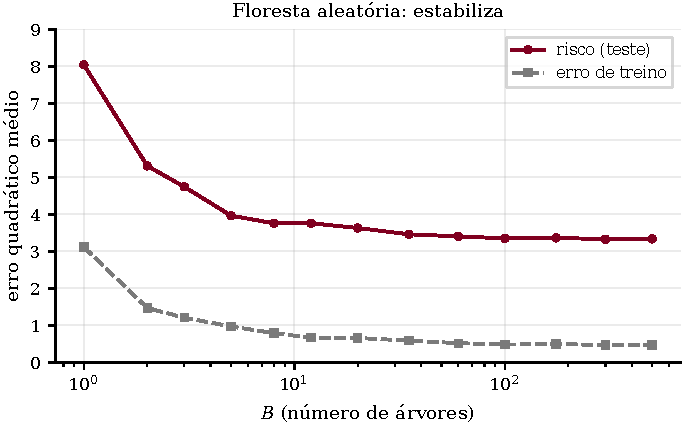
\includegraphics[width=\textwidth]{../../recursos/figuras/05-numero-arvores.pdf}
  \caption{A diferença mais prática entre os dois métodos, medida num problema com
  $n=150$, $p=8$ e ruído alto. À esquerda, a floresta: o risco cai, estabiliza em
  torno de $3{,}34$ e \emph{fica lá} --- de $B=100$ para $B=500$ ele varia $-0{,}4\%$.
  Você pode exagerar em $B$ à vontade; só perde tempo de máquina. À direita, o
  \emph{boosting} com $\lambda=0{,}05$: o risco atinge $3{,}23$ em $B=32$ e depois
  \textbf{volta a subir}, chegando a $3{,}75$ ($+16\%$) em $B=1500$, enquanto o erro
  de treino continua descendo rumo a zero. É o retrato do superajuste da Aula~01.}
  \label{fig:numeroarvores}
\end{figure}

\begin{atencao}
Diferença crucial em relação às florestas: no \emph{boosting}, $B$ \textbf{grande
demais superajusta}, como mostra a Figura~\ref{fig:numeroarvores}. Por isso o
\emph{early stopping} é essencial --- e por isso $B$ \emph{é} um hiperparâmetro no
\emph{boosting} e \emph{não é} nas florestas. Confundir os dois casos é um dos erros
mais comuns de quem está começando.
\end{atencao}

\begin{observacao}
A implementação moderna mais popular é o \textbf{XGBoost} (Chen \& Guestrin, 2016):
\emph{boosting} de árvores com regularização adicional, tratamento de dados
faltantes e altíssimo desempenho computacional --- frequentemente o melhor método
``pronto'' em dados tabulares.
\end{observacao}

%==============================================================================
\section{Prática em Python}
%==============================================================================
\begin{lstlisting}
from sklearn.tree import DecisionTreeRegressor
from sklearn.ensemble import RandomForestRegressor, GradientBoostingRegressor
from sklearn.model_selection import GridSearchCV

# Arvore unica: cuidado com superajuste -> controle a complexidade (alpha de poda)
arvore = DecisionTreeRegressor(ccp_alpha=0.0)   # ccp_alpha e o nosso alpha

# Floresta aleatoria: B grande, m = max_features (~ p/3 em regressao)
rf = RandomForestRegressor(n_estimators=500, max_features=1/3,
                           oob_score=True, random_state=0).fit(X_tr, y_tr)
print("risco OOB (R2):", rf.oob_score_)
print("importancias:", rf.feature_importances_)

# Boosting: lambda pequeno + B por early stopping
gb = GradientBoostingRegressor(learning_rate=0.01, n_estimators=2000,
                               max_depth=3, validation_fraction=0.2,
                               n_iter_no_change=20).fit(X_tr, y_tr)
\end{lstlisting}

\begin{observacao}
Três detalhes que fazem diferença nesse trecho. O \texttt{oob\_score=True} entrega a
estimativa OOB sem custo extra --- aproveite. Os argumentos
\texttt{validation\_fraction} e \texttt{n\_iter\_no\_change} são o \emph{early
stopping} do \texttt{scikit-learn}: sem eles, as 2000 árvores serão todas usadas, e
a Figura~\ref{fig:numeroarvores} mostra o que isso custa. E note que árvores
\textbf{não precisam} de \texttt{StandardScaler}: elas só comparam valores dentro de
cada variável, então a escala é irrelevante --- ao contrário do KNN da Aula~04.
\end{observacao}

O notebook \texttt{Aula prática 05} compara árvore, floresta e \emph{boosting} no
\texttt{superconductivity.csv}, e mede o piso $\rho\,v(\x)$ da variância.

%==============================================================================
\section*{Resumo}
%==============================================================================
\begin{itemize}[leftmargin=1.4cm]
  \item \textbf{Árvore}: partição recursiva \eqref{eq:arvore}, com os dois lados da
        Figura~\ref{fig:particao}; cresce gananciosamente \eqref{eq:split} e poda por
        custo--complexidade \eqref{eq:poda} ($\alpha$ por CV). Interpretável, mas
        alta variância, e só corta perpendicular aos eixos.
  \item Agregar reduz variância se os preditores são não-viesados e pouco
        correlacionados (Prop.~\ref{prop:media}); com correlação $\rho$, a variância
        trava em $\rho\,v(\x)$.
  \item \textbf{Bagging} \eqref{eq:bagging}: árvores profundas em amostras
        bootstrap; OOB ``de graça''; importância por redução de RSS (enviesada ---
        use com cuidado).
  \item \textbf{Florestas}: \emph{descorrelacionam} sorteando $m\approx p/3$
        variáveis por nó; robustas a $B$; adaptam-se à esparsidade.
  \item \textbf{Boosting}: ajuste sequencial dos resíduos, partindo do viés máximo;
        $\lambda$ pequeno, $p$ raso, $B$ por \emph{early stopping} --- aqui $B$
        grande \emph{superajusta} (Fig.~\ref{fig:numeroarvores}). XGBoost é a
        implementação de referência.
\end{itemize}

\paragraph{Leitura recomendada.} [AME] §4.8 (árvores, com o algoritmo de
crescimento e poda), §4.9 (\emph{bagging} e florestas aleatórias, incluindo a
importância de variáveis) e §4.10 (\emph{boosting}). [ISLP] Capítulo~8
(\emph{Tree-Based Methods}) --- §8.1 tem a versão deles da nossa
Figura~\ref{fig:particao}, e §8.2 compara \emph{bagging}, florestas e
\emph{boosting} nos mesmos dados.

\paragraph{Para praticar.} \texttt{Lista teorica 05.pdf} (teórica, com gabarito) e \texttt{Lista prática 05.ipynb} (prática, para completar as lacunas), nesta mesma pasta.

\end{document}
